% !TEX root = ../linal_lecture_01.tex

\begin{frame} % название фрагмента

\videotitle{Вектор: длина и скалярное произведение}

\end{frame}




\begin{frame}{Краткое напутствие}

%\uncover<1->{
    Зачем нужна \alert{линейная алгебра}?

\begin{itemize}[<+->]
  \item Линейная алгебра прекрасна сама по себе!
  \item Работает «под капотом» практически всех методов машинного обучения.
\end{itemize}

%}
\end{frame}



\begin{frame}{Краткий план:}
  \begin{itemize}[<+->]
    \item Вектор — это столбец чисел.
    \item Сложение двух векторов и умножение на число.
    \item Расстояние и косинус угла между векторами.
  \end{itemize}

\end{frame}


\begin{frame}{Вектор}


\begin{block}{Рабочее определение}
\alert{Вектор} — столбец из нескольких чисел.   

\[
\bv = \begin{pmatrix}
  \sqrt{5} \\
  3 \\
  -3.45
\end{pmatrix}
\]
\end{block}

\pause

\begin{block}{Идея вектора}
Вектор — всё, что можно описать столбцом из нескольких чисел. 
\end{block}

\pause
Мы не пишем стрелочку над вектором.

\pause
Вектор из нулей обозначаем $\bzero$.


\end{frame}



\begin{frame}{Пространство $\R^n$}

\begin{block}{Определение} 
\alert{Пространство $\R^n$:}

     Множество всех возможных векторов из $n$ чисел. 
 \[
 \R^n = \left\{ \begin{pmatrix}
 x_1 \\
 x_2 \\
 \vdots \\
 x_n \\
 \end{pmatrix} \middle| x_1 \in \R, \ldots, x_n \in \R
   \right\}  
 \]
\end{block}

\pause

\begin{block}{Определение} 
  \alert{Размерность} пространства $\R^n$:

    Количество чисел в каждом векторе, $n$.
\end{block}
\end{frame}







\begin{frame}{Длина вектора}




\begin{minipage}{0.3\textwidth}% adapt widths of minipages to your needs
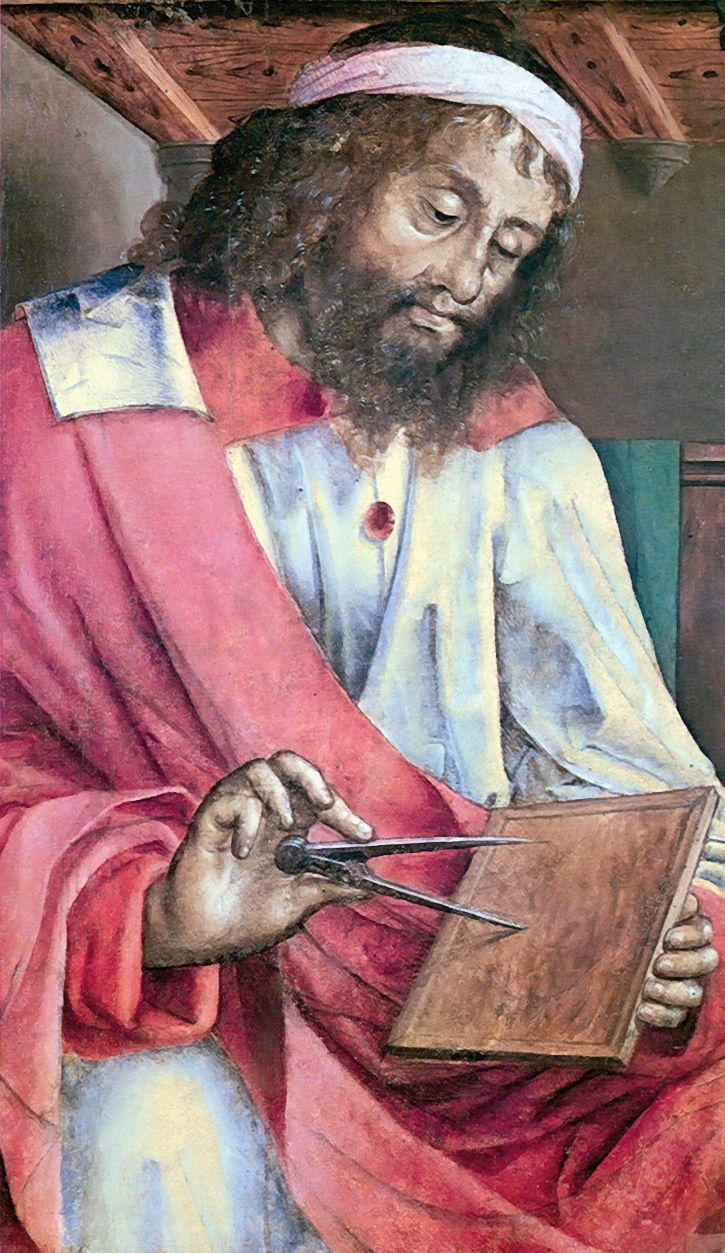
\includegraphics[scale=0.2]{figures/video_010_euklid.jpg}
\end{minipage}%
\hfill%
\begin{minipage}{0.6\textwidth}

\begin{block}{Определение} 
\alert{Евклидова длина} или \alert{норма} вектора 
\[
  \norm{\bx} = \sqrt{x_1^2 + x_2^2 + \ldots + x_n^2}.
\]
\end{block}
\end{minipage}

\figcaption{Евклид, около 300 лет до н.э.}

\graylink{wikipedia.org / общественное достояние}



\end{frame}



\begin{frame}{Длина вектора}
\begin{tikzpicture}[
scale=1.6,
MyPoints/.style={draw=blue,fill=white,thick},
Segments/.style={draw=blue!50!red!70,thick},
MyCircles/.style={green!50!blue!50,thin}, 
every node/.style={scale=1}
]
\grid;
\clip (-2.5,-2.5) rectangle (10.5,6.5);


%\draw[->, >=stealth] (-1,0)--(6.5,0) node[right]{$x_1$};
\draw[-{Latex[length=4.5mm, width=2.5mm]}, >=stealth] (0,-1)--(0,5) node[above left]{$x_2$};

\draw[-{Latex[length=4.5mm, width=2.5mm]}, >=stealth] (-1,0)--(6.5,0) 
node[right]{$x_1$};


%{\verb!->!new, arrowhead = 2mm, line width=4pt}
%, arrowhead = 3mm
%, arrowhead = 0.2

% Feel free to change here coordinates of points A and B
\pgfmathparse{0}		\let\Xa\pgfmathresult
\pgfmathparse{0}		\let\Ya\pgfmathresult
\coordinate (A) at (\Xa,\Ya);

\pgfmathparse{4}		\let\Xb\pgfmathresult
\pgfmathparse{3}		\let\Yb\pgfmathresult
\coordinate (B) at (\Xb,\Yb);

\pgfmathparse{4}		\let\Xc\pgfmathresult
\pgfmathparse{0}		\let\Yc\pgfmathresult
\coordinate (C) at (\Xc,\Yc);


% Let I be the midpoint of [AB]
\pgfmathparse{(\Xb+\Xa)/2} \let\XI\pgfmathresult
\pgfmathparse{(\Yb+\Ya)/2} \let\YI\pgfmathresult
\coordinate (I) at (\XI,\YI);	


\draw[-{Latex[length=4.5mm, width=2.5mm]}, >=stealth, vecb,thick] (A)--(B) node[midway,above]{$\bx$};

\draw[black, dashed, thick] (B)--(C) node[midway,right]{$3$};

\draw[black] (A)--(C) node[midway,below]{$4$};

\tkzMarkRightAngle[size=.3](A,C,B) 

\node [above right,darkgray] at (1,3.5) {$\bx=\left(\begin{array}{l}4 \\ 3\end{array}\right) \quad \|\bx\|=\sqrt{3^{2}+4^{2}}=5 $};

\end{tikzpicture}



\end{frame}




\begin{frame}{Сложение и вычитание двух векторов}

 \begin{block}{Определение} 
 \alert{Сложение и вычитание} двух векторов выполняем поэлементно:
    \[
    \begin{pmatrix}
      2 \\
      3.5 \\
      -1 
    \end{pmatrix} + \begin{pmatrix}
      3 \\
      -3 \\
      1 
    \end{pmatrix}  = \begin{pmatrix}
      5 \\
      0.5 \\
      0 
    \end{pmatrix}
    \]  
  \end{block}

\begin{tikzpicture}[
scale=1.2,
MyPoints/.style={draw=blue,fill=white,thick},
Segments/.style={draw=blue!50!red!70,thick},
MyCircles/.style={green!50!blue!50,thin}, 
every node/.style={scale=1.2}
]
%\grid;
%\clip (-.5,-.5) rectangle (5.5,5.5);


%%\draw[->, >=stealth] (-1,0)--(6.5,0) node[right]{$x_1$};
%\draw[-{Latex[length=4.5mm, width=2.5mm]}, >=stealth] (0,-1)--(0,5) node[above left]{$x_2$};
%
%\draw[-{Latex[length=4.5mm, width=2.5mm]}, >=stealth] (-1,0)--(6.5,0) 
%node[right]{$x_1$};

% Feel free to change here coordinates of points A and B
\pgfmathparse{0}		\let\Xa\pgfmathresult
\pgfmathparse{0}		\let\Ya\pgfmathresult
\coordinate (A) at (\Xa,\Ya);

\pgfmathparse{2}		\let\Xb\pgfmathresult
\pgfmathparse{4}		\let\Yb\pgfmathresult
\coordinate (B) at (\Xb,\Yb);

\pgfmathparse{3}		\let\Xc\pgfmathresult
\pgfmathparse{1}		\let\Yc\pgfmathresult
\coordinate (C) at (\Xc,\Yc);

\pgfmathparse{5}		\let\Xd\pgfmathresult
\pgfmathparse{5}		\let\Yd\pgfmathresult
\coordinate (D) at (\Xd,\Yd);



% Let I be the midpoint of [AB]
\pgfmathparse{(\Xb+\Xa)/2} \let\XI\pgfmathresult
\pgfmathparse{(\Yb+\Ya)/2} \let\YI\pgfmathresult
\coordinate (I) at (\XI,\YI);	


\draw[-{Latex[length=4.5mm, width=2.5mm]}, >=stealth, vecb,thick] (A)--(B) node[midway,left]{$\ba$};

\draw[-{Latex[length=4.5mm, width=1.5mm]}, >=stealth, vecb,dashed] (C)--(D) node[midway,right]{$\ba$};


\draw[-{Latex[length=4.5mm, width=2.5mm]}, >=stealth, veca,thick] (A)--(C) node[midway,below]{$\bb$};

\draw[-{Latex[length=4.5mm, width=1.5mm]}, >=stealth, veca,dashed] (B)--(D) node[midway,above]{$\bb$};


\draw[-{Latex[length=4.5mm, width=2.5mm]}, >=stealth, vecc,thick] (A)--(D) node[midway,above, sloped]{$\ba+\bb$};


\end{tikzpicture}


\end{frame}



\begin{frame}{Умножение вектора на число}


\begin{block}{Определение} 
\alert{Умножение} вектора на число выполняем поэлеметно:
    \[
    4 \cdot \begin{pmatrix}
      2 \\
      3.5 \\
      -1 
    \end{pmatrix} = \begin{pmatrix}
      8 \\
      14 \\
      -4 
    \end{pmatrix}  
    \]
  \end{block}


\begin{tikzpicture}[
  scale=1.2,
  MyPoints/.style={draw=blue,fill=white,thick},
  Segments/.style={draw=blue!50!red!70,thick},
  MyCircles/.style={green!50!blue!50,thin}, 
  every node/.style={scale=1.2}
  ]
  %\grid;
  %\clip (-.5,-.5) rectangle (5.5,5.5);

  \pgfmathparse{0}		\let\Xa\pgfmathresult
  \pgfmathparse{0}		\let\Ya\pgfmathresult
  \coordinate (A) at (\Xa,\Ya);

  \pgfmathparse{3}		\let\Xb\pgfmathresult
  \pgfmathparse{3}		\let\Yb\pgfmathresult
  \coordinate (B) at (\Xb,\Yb);

  \pgfmathparse{5}		\let\Xc\pgfmathresult
  \pgfmathparse{5}		\let\Yc\pgfmathresult
  \coordinate (C) at (\Xc,\Yc);

  \draw[-{Latex[length=4.5mm, width=2.5mm]}, >=stealth, black,thick] (A)--(C) node[above left]{$\lambda \cdot \ba$};

  \draw[-{Latex[length=4.5mm, width=2.5mm]}, >=stealth, veca,thick] (A)--(B) node[midway,above left]{$\ba$};


  \end{tikzpicture}


\end{frame}




\begin{frame}{Расстояние между векторами}

\begin{block}{Определение} 
\alert{Евклидово расстояние} между векторами
  \[
  d(\ba, \bb) = \norm{\ba - \bb} = \sqrt{(a_1 - b_1)^2 + \ldots + (a_n - b_n)^2}
  \]
\end{block}

\pause
По определению, $d(\ba, \bb) \geq 0$. 

Также говорят \alert{Евклидова метрика}.
\pause

\begin{tikzpicture}[
scale=1.2,
MyPoints/.style={draw=blue,fill=white,thick},
Segments/.style={draw=blue!50!red!70,thick},
MyCircles/.style={green!50!blue!50,thin}, 
every node/.style={scale=1.2}
]
%\grid;
%\clip (-.5,-.5) rectangle (5.5,5.5);


%%\draw[->, >=stealth] (-1,0)--(6.5,0) node[right]{$x_1$};
%\draw[-{Latex[length=4.5mm, width=2.5mm]}, >=stealth] (0,-1)--(0,5) node[above left]{$x_2$};
%
%\draw[-{Latex[length=4.5mm, width=2.5mm]}, >=stealth] (-1,0)--(6.5,0) 
%node[right]{$x_1$};

% Feel free to change here coordinates of points A and B
\pgfmathparse{0}		\let\Xa\pgfmathresult
\pgfmathparse{0}		\let\Ya\pgfmathresult
\coordinate (A) at (\Xa,\Ya);

\pgfmathparse{1}		\let\Xb\pgfmathresult
\pgfmathparse{4}		\let\Yb\pgfmathresult
\coordinate (B) at (\Xb,\Yb);

\pgfmathparse{3}		\let\Xc\pgfmathresult
\pgfmathparse{1}		\let\Yc\pgfmathresult
\coordinate (C) at (\Xc,\Yc);




% Let I be the midpoint of [AB]
\pgfmathparse{(\Xb+\Xa)/2} \let\XI\pgfmathresult
\pgfmathparse{(\Yb+\Ya)/2} \let\YI\pgfmathresult
\coordinate (I) at (\XI,\YI);	


\draw[-{Latex[length=4.5mm, width=2.5mm]}, >=stealth, vecb,thick] (A)--(B) node[midway,left]{$\ba$};


\draw[-{Latex[length=4.5mm, width=2.5mm]}, >=stealth, veca,thick] (A)--(C) node[midway,below]{$\bb$};


\draw[-{Latex[length=4.5mm, width=2.5mm]}, >=stealth, vecc,thick] (C)--(B) node[midway,right]{$\ba-\bb$};


\end{tikzpicture}
    


\end{frame}






\begin{frame}{Скалярное произведение и угол}

\begin{block}{Определение} 
\alert{Скалярное произведение} векторов $\ba$ и $\bb$:

  \[
    \langle \ba, \bb \rangle = a_1 b_1 + a_2 b_2 + \ldots + a_n b_n.
  \]
\end{block}
\pause

\begin{block}{Определение} 
\alert{Косинус угла} и \alert{угол} между векторами $\ba$ и $\bb$:
% Косинусная близость, cosine similarity:  
  \[
  \cos \angle (\ba, \bb) =  \frac{\langle \ba, \bb \rangle}{ \norm{\ba} \norm{\bb}} \quad   \angle (\ba, \bb) =  \arccos \frac{\langle \ba, \bb \rangle}{ \norm{\ba} \norm{\bb}} 
  \]
\end{block}

Угол определён, если $\norm{\ba} > 0$ и $\norm{\bb} > 0$.


\begin{tikzpicture}[
scale=1.2,
MyPoints/.style={draw=blue,fill=white,thick},
Segments/.style={draw=blue!50!red!70,thick},
MyCircles/.style={green!50!blue!50,thin}, 
every node/.style={scale=1.2}
]
%\grid;

%\clip (-.5,-.5) rectangle (6.5,5.5);


%%\draw[->, >=stealth] (-1,0)--(6.5,0) node[right]{$x_1$};
%\draw[-{Latex[length=4.5mm, width=2.5mm]}, >=stealth] (0,-1)--(0,5) node[above left]{$x_2$};
%
%\draw[-{Latex[length=4.5mm, width=2.5mm]}, >=stealth] (-1,0)--(6.5,0) 
%node[right]{$x_1$};

% Feel free to change here coordinates of points A and B
\pgfmathparse{0}		\let\Xa\pgfmathresult
\pgfmathparse{0}		\let\Ya\pgfmathresult
\coordinate (A) at (\Xa,\Ya);

\pgfmathparse{1}		\let\Xb\pgfmathresult
\pgfmathparse{4}		\let\Yb\pgfmathresult
\coordinate (B) at (\Xb,\Yb);

\pgfmathparse{4}		\let\Xc\pgfmathresult
\pgfmathparse{1}		\let\Yc\pgfmathresult
\coordinate (C) at (\Xc,\Yc);


\draw[-{Latex[length=4.5mm, width=2.5mm]}, >=stealth, vecb,thick] (A)--(B) node[midway,left]{$\ba$};


\draw[-{Latex[length=4.5mm, width=2.5mm]}, >=stealth, veca,thick] (A)--(C) node[midway,below]{$\bb$};


\tkzMarkAngle[size=1, mark = none](C,A,B);

\node [darkgray] at (1,1) {$\varphi$}; 

% \node [above right, darkgray] at (2, 2) {$\cos \varphi=\dfrac{\langle \ba, \bb\rangle}{\|\ba\| \cdot\|\bb\|}$}; 

%\draw
%(3,-1) coordinate (a) node[right] {$a$}
%-- (0,0) coordinate (b) node[left] {b}
%-- (2,2) coordinate (c) node[above right] {c}


\end{tikzpicture}
  




  


\end{frame}





\begin{frame}{Свойства скалярного произведения}

  
  \begin{itemize}[<+->]
  \item Скалярное произведение вектора на себя равно квадрату длины
  $\langle \ba, \ba \rangle = \norm{\ba}^2$

  \item Линейность по каждому аргументу
  $\langle \lambda \ba, \bb \rangle = \langle \ba,  \lambda  \bb \rangle = \lambda  \langle \ba,  \bb \rangle$

  $\langle \ba + \bb, \bc \rangle = \langle \ba , \bc \rangle + \langle \bb , \bc \rangle$

  \item Симметричность
  
  $\langle \ba, \bb \rangle = \langle \bb, \ba \rangle$

  \item Скалярное произведение для ненулевых векторов
  
  $\langle \ba, \bb \rangle = \norm{\ba}\norm{\bb} \cos \angle(\ba, \bb)$
  \end{itemize}
  
  

\end{frame}




\begin{frame}{Скалярное произведение и проекция}

\begin{itemize}[<+->]
  \item Следствие формулы $\langle \ba, \bb \rangle = \norm{\ba}\norm{\bb} \cos \angle(\ba, \bb)$

\item Если вектор $\ba$ имеет единичную длину, $\norm{\ba} = 1$, то 


$\langle \ba, \bb \rangle = \norm{\bb} \cos  \angle(\ba, \bb)$ — длина$^*$ проекции $b$ на $a$.
  


\begin{tikzpicture}[
  scale=1.2,
  MyPoints/.style={draw=blue,fill=white,thick},
  Segments/.style={draw=blue!50!red!70,thick},
  MyCircles/.style={green!50!blue!50,thin}, 
  every node/.style={scale=1.2}
  ]
  %\grid;
  
  %\clip (-1.5,-1.5) rectangle (7.5,5.5);
  
  
  %%\draw[->, >=stealth] (-1,0)--(6.5,0) node[right]{$x_1$};
  %\draw[-{Latex[length=4.5mm, width=2.5mm]}, >=stealth] (0,-1)--(0,5) node[above left]{$x_2$};
  %
  %\draw[-{Latex[length=4.5mm, width=2.5mm]}, >=stealth] (-1,0)--(6.5,0) 
  %node[right]{$x_1$};
  
  % Feel free to change here coordinates of points A and B
  \pgfmathparse{0}		\let\Xa\pgfmathresult
  \pgfmathparse{0}		\let\Ya\pgfmathresult
  \coordinate (A) at (\Xa,\Ya);
  
  \pgfmathparse{5.5}		\let\Xb\pgfmathresult
  \pgfmathparse{5.5}		\let\Yb\pgfmathresult
  \coordinate (B) at (\Xb,\Yb);
  
  \pgfmathparse{5}		\let\Xc\pgfmathresult
  \pgfmathparse{2}		\let\Yc\pgfmathresult
  \coordinate (C) at (\Xc,\Yc);
  
  \pgfmathparse{-1}		\let\Xd\pgfmathresult
  \pgfmathparse{1}		\let\Yd\pgfmathresult
  \coordinate (D) at (\Xd,\Yd);
  
  \pgfmathparse{3}		\let\Xe\pgfmathresult
  \pgfmathparse{5}		\let\Ye\pgfmathresult
  \coordinate (E) at (\Xe,\Ye);
  
  \pgfmathparse{-0.75}		\let\Xf\pgfmathresult
  \pgfmathparse{0.75}		\let\Yf\pgfmathresult
  \coordinate (F) at (\Xf,\Yf);
  
  \pgfmathparse{3.25}		\let\Xg\pgfmathresult
  \pgfmathparse{4.75}		\let\Yg\pgfmathresult
  \coordinate (G) at (\Xg,\Yg);
  
  \pgfmathparse{4}		\let\Xh\pgfmathresult
  \pgfmathparse{4}		\let\Yh\pgfmathresult
  \coordinate (H) at (\Xh,\Yh);
  
  \pgfmathparse{6}		\let\Xj\pgfmathresult
  \pgfmathparse{2}		\let\Yj\pgfmathresult
  \coordinate (J) at (\Xj,\Yj);
  
  \draw[-{Latex[length=4.5mm, width=2.5mm]}, >=stealth, vecb,thick] (A)--(B) node[midway,left]{$\ba$};
  
  
  \draw[-{Latex[length=4.5mm, width=2.5mm]}, >=stealth, veca,thick] (A)--(J) node[midway,below]{$\bb$};
  
  \draw[thick] (A)--(D);
  \draw[thick] (H)--(E);
  
  \draw[thick, dashed] (J)--(E);
  
  
  \draw[{Latex[length=4.5mm, width=2.5mm]}-{Latex[length=4.5mm, width=2.5mm]}, >=stealth, thick] (F)--(G) node[midway,above left]{$\langle \ba, \bb \rangle$};
  
  
  
  
  \tkzMarkRightAngle[size=0.3, mark = none](A,H,J);
  
  \tkzMarkAngle[size=1, mark = none](C,A,B);
  
  
  %\node [below, darkgray] at (1,1) {$\varphi$}; 
  
  %\node [below right, darkgray] at (-1.5,-1) {если  $\| \ba \| = 1 $, то $\langle \ba, \bb \rangle$  -- длина* проекции $\bb$ на $\ba$}; 
  
  
  
  %\draw
  %(3,-1) coordinate (a) node[right] {$a$}
  %-- (0,0) coordinate (b) node[left] {b}
  %-- (2,2) coordinate (c) node[above right] {c}
  
  
  \end{tikzpicture}
  


\end{itemize}

  



\end{frame}





% \begin{frame}{Почти любой объект — вектор!}

%   \begin{block}{С помощью вектора можно закодировать:}
%   \begin{itemize}
%     \item многочлен 
%     \[
%     3x^2 + 6 x - 7 \to (3, 6, -7)  
%     \]
%     \item характеристики индивида

%     \[
%     \text{Блондин с ростом 182 см и весов 81 килограмм} \to (0, 182, 81)
%     \]
%     \item TODO
%   \end{itemize}

%   \end{block}
% \end{frame}




\begin{frame}{Ортогональность векторов}

\begin{block}{Определение}
Векторы $\ba$ и $\bb$ \alert{ортогональны}, $a\perp b$, если
\[
  \langle \ba, \bb \rangle =0
\]
\end{block}

Также говорят «\alert{перпендикулярны}».

\end{frame}


\begin{frame}{Ортогональность векторов}

Для ненулевых векторов $\langle \ba, \bb \rangle \norm{\ba}\norm{\bb}\cos\angle(\ba, \bb) = 0$: 


\begin{tikzpicture}[
scale=1.6,
MyPoints/.style={draw=blue,fill=white,thick},
Segments/.style={draw=blue!50!red!70,thick},
MyCircles/.style={green!50!blue!50,thin}, 
every node/.style={scale=1.2}
]
%\grid;

\clip (-2,-1.5) rectangle (10.5,5.5);


%%\draw[->, >=stealth] (-1,0)--(6.5,0) node[right]{$x_1$};
%\draw[-{Latex[length=4.5mm, width=2.5mm]}, >=stealth] (0,-1)--(0,5) node[above left]{$x_2$};
%
%\draw[-{Latex[length=4.5mm, width=2.5mm]}, >=stealth] (-1,0)--(6.5,0) 
%node[right]{$x_1$};

% Feel free to change here coordinates of points A and B
\pgfmathparse{0}		\let\Xa\pgfmathresult
\pgfmathparse{0}		\let\Ya\pgfmathresult
\coordinate (A) at (\Xa,\Ya);

\pgfmathparse{1}		\let\Xb\pgfmathresult
\pgfmathparse{4}		\let\Yb\pgfmathresult
\coordinate (B) at (\Xb,\Yb);

\pgfmathparse{4}		\let\Xc\pgfmathresult
\pgfmathparse{-1}		\let\Yc\pgfmathresult
\coordinate (C) at (\Xc,\Yc);

\pgfmathparse{-1}		\let\Xc\pgfmathresult
\pgfmathparse{4}		\let\Yc\pgfmathresult
\coordinate (D) at (\Xc,\Yc);



\draw[-{Latex[length=4.5mm, width=2.5mm]}, >=stealth, vecb,thick] (A)--(B) node[above left]{$\ba$};


\draw[-{Latex[length=4.5mm, width=2.5mm]}, >=stealth, veca,thick] (A)--(C) node[above right]{$\bb$};

\draw[-{Latex[length=4.5mm, width=2.5mm]}, >=stealth, thick] (A)--(D) node[above left]{$\bc$};


\tkzMarkRightAngle[size=0.5](C,A,B);


\node [above right, darkgray] at (2, 2) {$\ba\perp \bb$ и $\ba\nperp \bc$}; 



%\draw
%(3,-1) coordinate (a) node[right] {$a$}
%-- (0,0) coordinate (b) node[left] {b}
%-- (2,2) coordinate (c) node[above right] {c}


\end{tikzpicture}


\end{frame}



    